\section{Introduction motivante : l'équation de la chaleur}

Intéressons-nous au problème monodimensionnel de la propagation de la chaleur dans une barre métallique longue de 1 m. 
Un point de cette barre est repéré par une abscisse $x$ allant de 0 à 1. On note $T(x,t)$ la température de la barre au 
point d'abscisse $x$ et au temps $t$. Le problème comporte également deux conditions dites \emph{aux limites} : pour 
tout $t\in\R$, les températures $T(0,t)$ et $T(1,t)$ sont fixes et notées $T_g$ et $T_d$. Il comporte également une 
condition initiale : pour $t=0$, l'ensemble de la barre et à la température $T_0$, \emph{i.e.} pour tout $x\in[0,1]$, 
$T(x,0)=T_0$.

%\clearslide{}

La modélisation physique classique permet d'aboutir à une \emph{équation aux dérivées partielles} (EDP) vérifiée par 
$T$, et appelée \emph{équation de la chaleur} :
$$\dfrac{\partial T}{\partial t}=\alpha\dfrac{\partial^2T}{\partial x^2}\ ,$$
où $\alpha$ est la \emph{diffusivité thermique.}

%\clearslide{}

L'intervalle $[0,1]$ est subdivisé en $N$ sous-intervalles de longueur constante $h_x=\frac1N$. Pour tout 
$i\in\llbr 0,N\rrbr$, on note $x_i=ih$. On dit qu'on a \emph{discrétisé} ou \emph{maillé} l'intervalle $[0,1]$ : les 
points $x_i$ sont appelés les \emph{n\oe uds} du maillage, et les intervalles $[x_i,x_{i+1}]$ en sont les 
\emph{cellules}.

Le temps est également discrétisé en sous-intervalles de longueur $h_t$ : $h_t$ est donc le \emph{pas temporel}, et 
$h_x$ le \emph{pas spatial}. Nous noterons alors $T_i^n$ la température au point d'abscisse $x_i$ et au temps $t=nh_t$. 
Par extension, pour toute fonction $\varphi$, $\varphi_i^n$ désignera la valeur de $\varphi$ au point d'abscisse $x_i$ 
et au temps $t=nh_t$.

%\clearslide{}

Comme pour la méthode d'Euler, nous allons approcher les dérivées intervenant dans l'équation de la chaleur en 
utilisant des taux d'acccroissement, ce qui permettra, en connaissant les $T_i^n$ pour tout $i$ et à un certain $n$, 
d'en déduire une relation de récurrence donnant les $T_i^{n+1}$, pour tout $i$.

En toute rigueur, les $T_i^n$ ne désigneront pas la valeur exacte de $T(x_i,nh_t)$, que nous ne savons pas calculer, 
mais une approximation.

Là aussi, il existe deux approximations classiques des dérivées, menant à deux schémas numériques différents : le 
schéma \emph{explicite} et le schéma \emph{implicite}.

%\clearslide{}

\subsection{Le schéma explicite}

Voici les approximations utilisées :
$$\p{\dfrac{\partial T}{\partial t}}_i^n=\dfrac{T_i^{n+1}-T_i^n}{h_t}$$
et
$$\p{\dfrac{\partial^2T}{\partial x^2}}_i^n=\dfrac{\dfrac{T_{i+1}^n-T_i^n}{h_x}-\dfrac{T_i^n-T_{i-1}^n}{h_x}}{h_x}=
\dfrac{T_{i+1}^n-2T_i^n+T_{i-1}^n}{h_x^2}.$$

%\clearslide{}

En posant $\lambda = \alpha\dfrac{h_t}{h_x^2}$, la température à l'itération $n+1$ est donnée, pour tout 
$i\in\llbr1,N-1\rrbr$, par :

$$ T_i^{n+1} = \lambda T_{i-1}^n+(1-2\lambda)T_i^n+ \lambda T_{i+1}^n$$

%\clearslide{}

Ou encore, sous forme matricielle :

$$\begin{pmatrix} T_1\\T_2\\ \vdots \\T_{N-2}\\ T_{N-1} \end{pmatrix} ^{n+1} = 
\begin{pmatrix}1-2\lambda & \lambda 	& 0 		& \cdots 	& 0 \\
\lambda 	& 1-2\lambda 	& \lambda 	& \cdots 	& 0\\
\vdots		& \ddots 	& \ddots 	& \ddots 	& \vdots \\
0		& 0		& \lambda 	& 1-2\lambda 	& \lambda \\
0		& 0		& 0		& \lambda 	& 1-2\lambda \end{pmatrix}
\begin{pmatrix} T_1\\T_2\\ \vdots \\T_{N-2}\\ T_{N-1} \end{pmatrix} ^{n} + \lambda \begin{pmatrix} T_g\\ 0\\ \vdots \\ 
0\\ T_d \end{pmatrix}.$$

\subsection{Le schéma implicite}

Voici les approximations utilisées :
$$\p{\dfrac{\partial T}{\partial t}}_i^{n+1}=\dfrac{T_i^{n+1}-T_i^n}{h_t}$$
et
$$\p{\dfrac{\partial^2T}{\partial 
x^2}}_i^{n+1}=\dfrac{\dfrac{T_{i+1}^{n+1}-T_i^{n+1}}{h_x}-\dfrac{T_i^{n+1}-T_{i-1}^{n+1}}{h_x}}{h_x}=
\dfrac{T_{i+1}^{n+1}-2T_i^{n+1}+T_{i-1}^{n+1}}{h_x^2}.$$

%\clearslide{}

En posant $\lambda = \alpha\dfrac{h_t}{h_x^2}$, la température à l'itération $n+1$ est donnée, pour tout 
$i\in\llbr1,N-1\rrbr$, par :

$$ (1+2\lambda)T_i^{n+1}- \lambda (T_{i+1}^{n+1}+T_{i-1}^{n+1}) = T_i^n$$

%\clearslide{}

Ou encore, sous forme matricielle :

$$\begin{pmatrix}1+2\lambda & -\lambda 	& 0 		& \cdots 	& 0 \\
-\lambda 	& 1+2\lambda 	& -\lambda 	& \cdots 	& 0\\
\vdots		& \ddots 	& \ddots 	& \ddots 	& \vdots \\
0		& 0		& -\lambda 	& 1+2\lambda 	& -\lambda \\
0		& 0		& 0		& -\lambda 	& 1+2\lambda \end{pmatrix}
\begin{pmatrix} T_1\\T_2\\ \vdots \\T_{N-2}\\ T_{N-1} \end{pmatrix} ^{n+1} =
\begin{pmatrix} T_1\\T_2\\ \vdots \\T_{N-2}\\ T_{N-1} \end{pmatrix} ^{n} + \lambda \begin{pmatrix} T_g\\ 0\\ \vdots \\ 
0\\ T_d \end{pmatrix}.$$

%\clearslide{}

Les choses ne sont donc pas aussi directes que lors de l'utilisation du schéma explicite : un simple produit matriciel 
ne suffit pas pour passer de la $n\ieme$ itération à la $(n+1)\ieme$, il faut ici \emph{résoudre un système linéaire}.

On pourrait être tenté d'écarter le schéma implicite pour éviter ce problème, mais il se trouve que ce schéma présente 
de qualité de \emph{stabilité} que n'a pas le schéma explicite : il permet d'utiliser des pas de temps plus grands 
(donc de diminuer la taille de la matrice) sans trop altérer la qualité du résultat, et est plus tolérant face aux 
erreurs d'approximation. Il est donc très utilisé en pratique, en particulier pour étudier des phénomènes lents sur de 
grandes plages de temps.

%\clearslide{}
Ici le problème est monodimensionnel, mais il existe des problèmes en dimension 2 ou 3. Par exemple en dimension 3, les 
dérivées partielles peuvent se faire selon $x$, $y$, $z$ ou $t$. On rajoute un second et un troisième pas 
d'espace : $h_y$ et $h_z$. Le domaine spatial d'étude est alors maillé par des parallélépipèdes. Mais le principe de 
base reste le même.

On peut également mailler le domaine par des triangles, des tétraèdres, ou toute autre forme géométrique (voir les figures~\ref{fig:carcrash} et~\ref{fig:eqelectromag} pour des illustrations).

%\clearslide{}

Exemples :

\begin{itemize}
\item Diffusion de la chaleur dans un matériau ;
\item Calcul du champ magnétique induit par une source électromagnétique ;
\item Simulation de déformation d'une voiture en cas de choc ;
\item Prévisions météorologiques ;
\item \ldots{}
\end{itemize}

\begin{figure}
\begin{center}
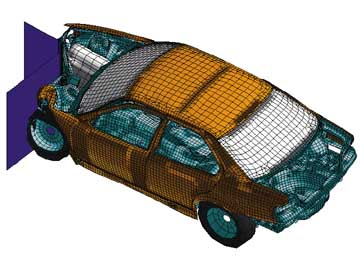
\includegraphics[width=0.7\textwidth]{FEM_car_crash1.jpg}  
\caption{Maillage utilisé pour simuler la déformation d'une voiture lors d'une collision.}
\label{fig:carcrash}
\end{center}
\end{figure}
% \text{Im}mediate\write\tempfile{FEM car crash1.jpg sur Wikimedia Commons,
%   licence CC-BY-SA-3.0, Pso.
% }
%\clearslide{}


\begin{figure}
\begin{center}
  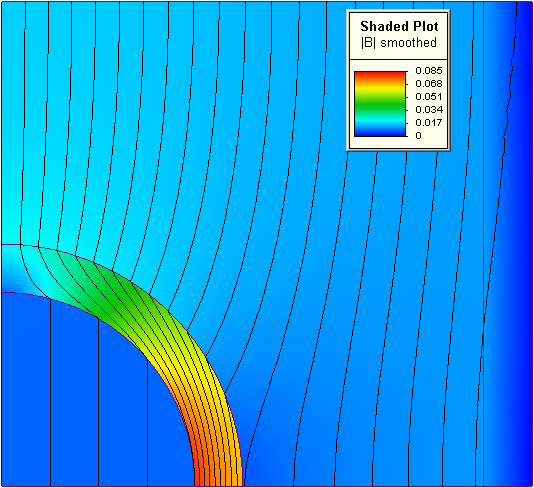
\includegraphics[width=0.4\textwidth]{FEM_example_of_2D_solution.png}
  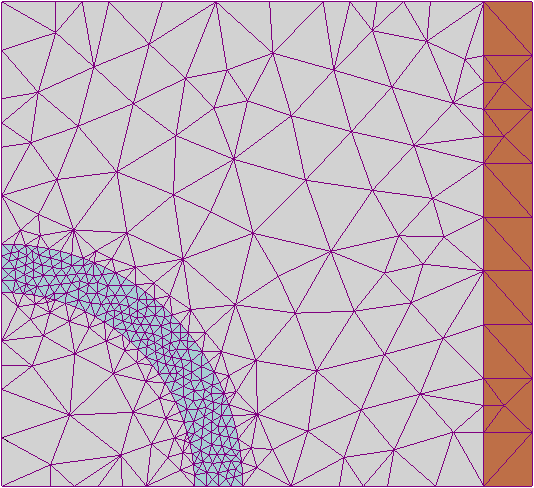
\includegraphics[width=0.4\textwidth]{Example_of_2D_mesh.png}
  \caption{Solution d'une équation magnétostatique. À droite, le maillage utilisé.}
  \label{fig:eqelectromag}
\end{center}
\end{figure}
% \text{Im}mediate\write\tempfile{Images: FEM example of 2D solution.png
%   Example of 2D mesh.png sur Wikimedia Commons, licence CC-BY-SA-3.0}
% \begin{filecontents}{credits.tex}
% à\tiny{
% }
% \end{filecontents}


%\clearslide{}

Dans le cas de prévisions météorologiques sur de grandes échelles d'espace et / ou de temps, le nombre de noeuds du 
maillage peut être énorme, parfois plusieurs milliers. D'où l'importance de disposer d'algorithmes efficaces de 
résolution de systèmes linéaires.

Comme sur l'exemple de l'équation de la chaleur, les matrices considérées sont souvent \emph{creuses} (elles 
contiennent beaucoup plus de zéros qu'autre chose), ce qui peut être exploité.

%\clearslide{}

\section{Méthode de Gauss-Jordan}

On l'appelle aussi \og méthode du pivot de Gauss\fg\ : c'est celle qui a été vue en mathématiques ! 
Lorsqu'on résout un système \og à la main \fg, on ne la suit pas forcément à la lettre.
Nous allons la détailler d'un point de vue algorithmique. 

On veut résoudre l'équation $Ax = b$, où $A = (a_{i,j}) \in\cM_{n}(\K)$ et $b = (b_i) \in \cM_{n1}(\K)$ sont donnés,
d'inconnue $x = (x_i) \in \cM_{n1}(\K)$. Cette équation se voit naturellement comme le système linéaire suivant.
\begin{equation}\label{eq:systeme}\tag{$\cS$}
  \left\{\begin{array}{cccccccccccc} 
a_{1,1} x_1 & + & \dots & + & a_{1,j}x_j & + & \dots & + & a_{1,n} x_n & = & b_1 \\ 
     \vdots &   &       &   & \vdots     &   &       &   & \vdots      &   &\vdots \\ 
a_{i,1} x_1 & + & \dots & + & a_{i,j}x_j & + & \dots &   & a_{i,n} x_n & = & b_i \\ 
     \vdots &   &       &   & \vdots     &   &       &   & \vdots      &   &\vdots \\ 
a_{n,1} x_1 & + & \dots & + & a_{n,j}x_j & + & \dots & + & a_{n,n} x_n & = & b_n  
\end{array}\right.
\end{equation}


\subsection{Cas où $A$ est triangulaire}

Si $A$ est triangulaire (par exemple supérieure) et inversible (ce qui équivaut à $\forall
k,~a_{kk}\neq 0$), la résolution est facile. Le système \eqref{eq:systeme} s'écrit alors plus simplement. 
\begin{equation*}
\left\{\begin{array}{ccccccccccc}
  a_{11}x_{1} &+& a_{12}x_{2} &+& \cdots &+& \cdots&+& a_{1n}x_{n} &=& b_{1}\\
  && a_{22} x_{2}&+ & \cdots &+& \cdots&+&a_{2n}x_{n}& = &b_{2}\\
  & &&\ddots & & & \vdots && \vdots & &\vdots\\
  &&&& a_{kk}x_{k}&+&\cdots&+&a_{kn}x_{n}&=&b_{k}\\
  &&&&      &\ddots &\vdots&&\vdots& & \vdots\\
  &&&&      &       &      &&a_{nn}x_{n}&=&b_{n}
\end{array} \right. 
\end{equation*}
%\clearslide{}
Les solutions de \eqref{eq:systeme} se calculent de proche en proche de la manière suivante. 
\begin{align*}
  x_{n} &= \frac{1}{a_{nn}}\p{b_{n}}\\
  x_{n-1} &= \frac{1}{a_{n-1,n-1}}\p{b_{n-1}-a_{n-1, n}x_{n}}\\
 & \vdots\\
  x_{k} &= \frac{1}{a_{k,k}}\p{b_{k}-a_{k,k+1}x_{k+1}-\cdots -a_{k,n}x_{n}}\\
\end{align*}

%On code ce système avec une matrice $N\in\cM_{n,n+1}(\  K)$ obtenue en
%accolant $\cM$ et $b$.

\subsection{Cas général}

On suppose que le système (\emph{i.e.} $A$) est carré ainsi qu'inversible.
On se ramène au cas triangulaire : pour cela on va effectuer des
opérations sur les lignes du système $Ax = b$. Ces opérations sont 
\begin{itemize}
  \item des échanges de lignes,
  \item des ajouts à une ligne de combinaisons linéaires d'autres lignes.
\end{itemize}
On peut voir chacune de ces opérations comme une opération matricielle, via la multiplication à gauche de matrices 
d'échange et de transvection.

\begin{exemple}[Matrice d'échange]
  Soit 
 \begin{equation*}
   E_{1,3} =
   \begin{pmatrix}
     0 & 0 & 1 & 0\\
     0 & 1 & 0 & 0\\
     1& 0 & 0 & 0\\
     0 & 0 & 0 & 1\\
   \end{pmatrix}.
 \end{equation*}
  Soit $B$ une matrice ayant $4$ lignes $L_{1}$, $L_{2}$, $L_{3}$, $L_{4}$. 
 Alors, $E_{1,3}B$ a les mêmes lignes que $B$ sauf la $3\ieme$ ligne qui est $L_{1}$ et la première 
ligne qui est $L_{3}$. Multiplier $B$ à gauche par $E_{1,3}$ revient donc à effectuer l'opération $L_1 \leftrightarrow L_3$.
\end{exemple}

\begin{exemple}[Matrice de transvection]
  Soit
   \begin{equation*}
   T_{\lambda} =
   \begin{pmatrix}
     1 & 0 & 0 & 0\\
     0 & 1 & 0 & 0\\
     \lambda & 0 & 1 & 0\\
     0 & 0 & 0 & 1\\
   \end{pmatrix}.
 \end{equation*}
 Soit $B$ une matrice ayant $4$ lignes $L_{1}$, $L_{2}$, $L_{3}$, $L_{4}$.
 Alors, $T_{1,3,\lambda}B$ a les mêmes lignes que $B$ sauf la $3$\up{e} ligne qui est $L_{3}
 + \lambda L_{1}$.
\end{exemple}
 
\begin{defi}[Matrice de transvection] 
  Soit $n\in\N^\ast$, $i,j \in \iif{1,n}$ avec $i\neq j$, soit $\lambda \in \R$. La matrice de transvection $T_{i,j,\lambda}$ est $I_n + \lambda E_{i,j}$, où $E_{i,j}$ est la matrice élémentaire nulle, hormis le coefficient d'indice $(i,j)$ qui vaut $1$.
  
  Ainsi, $T_{i,j,\lambda}$ correspond à la matrice identité, sauf pour son coefficient d'indice $(i,j)$ qui vaut $\lambda$.
\end{defi}
 
 %\clearslide{}
 
Numérotons, suivant notre habitude pythonesque, les lignes de $0$ à $n-1$ et les colonnes de $0$ à
$n-1$, notons $L_{i}$ la $i\ieme$ ligne  de $A$ pour chaque $i\in\ii{0,n}$.
L'algorithme du pivot est le suivant:
%\clearslide{}
\begin{enumerate}
\item Phase de \emph{descente} : pour chaque $i=0, 1, \ldots, n-1$.
  \begin{enumerate}
  \item\label{partiel} Trouver $j$ dans $\ii{i, n}$ tel que $a_{ji}$ soit non nul (c'est toujours 
possible, car le système est inversible).
  \item Échanger les lignes $i$ et $j$ dans $A$ et dans $b$.
  \item Poser $p = a_{ii}$ (c'est le \emph{pivot}).
  \item Pour $j$ de $i+1$ à $n-1$:
    \begin{enumerate}
    \item Remplacer $b_{j}$ par $b_{j}-\frac{a_{ji}}{p}b_{i}$.
    \item Remplacer la ligne $L_{j}$ de $A$ par $L_{j} - \frac{a_{ji}}{p}L_{i}$.
    \end{enumerate}
  \end{enumerate}
\item Phase de \emph{remontée} : $A$ est maintenant triangulaire, on peut calculer la solution avec la méthode précédente.
\end{enumerate}

\begin{rem}
  Cet algorithme modifie la matrice $A$ ainsi que le vecteur $b$. En pratique, on l'effectuera après avoir recopié les données. 
\end{rem}



Attention : se contenter de choisir un pivot non nul peut être problématique.
Par exemple, un 
coefficient devrait être nul après un certain nombre de calculs. 
À cause d'erreurs d'arrondis, il 
est représenté par un coefficient non nul, et peut être choisi comme pivot. 
Ou bien, à cause d'erreurs d'arrondis, un coefficient qui devait-être non nul est représenté comme le flottant nul. 
Le système n'est alors plus inversible ! 

Pour palier cela, on utilise la méthode du \emph{pivot partiel}. 
Il suffit de remplacer l'étape \ref{partiel}) par la suivante. 
\begin{center}
Trouver $j$ dans $\ii{i, n}$ tel que $\abs{a_{ji}}$ soit maximale.
\end{center}


%\clearslide{}
\section{Matrices avec \texttt{numpy}.}

Nous représenterons les matrices par des tableaux bidimensionnels, en utilisant le type \texttt{array} de la bibliothèque \texttt{numpy}. 

\begin{pyconsole}
from numpy import array
M = array([[1.,2.,3.],[4.,5.,6.],[7.,8.,9.],[10.,11.,12.]])
M
\end{pyconsole}
On remarquera notamment que les matrices sont décrites ligne par ligne. 
On peut accéder à un coefficient de la matrice par un double indice. 
\begin{pyconsole}
M[0,0]
M[1,2]
\end{pyconsole}
Il est aussi possible d'extraire une ou des lignes
\begin{pyconsole}
M[[0],:]
M[[1,2],:]
\end{pyconsole}
De même, il est possible d'extraire une ou plusieurs colonnes d'une matrice. 
\begin{pyconsole}
M[:,[1]]
M[:,[0,2]]
\end{pyconsole}
\begin{rem}
Il est aussi possible d'extraire une sous-matrice de $M$. 
\end{rem}
On peut obtenir les dimensions de d'une matrice par la méthode \texttt{shape}.
\begin{pyconsole}
M.shape
\end{pyconsole}
\begin{rem}
Attention, les commandes suivantes extraient bien une ligne ou une colonne d'une matrice, mais ne renvoient pas un résultat sous forme de matrice, mais de vecteurs. 
\begin{pyconsole}
M[0,:]
M[:,0]
\end{pyconsole}
C'est toutefois très pratique pour effectuer des opérations sur les lignes et les colonnes de $M$.
\begin{pyconsole}
L = array([42.,42.,42.])
M[0,:] = M[0,:] + L
M
\end{pyconsole}
\end{rem}
Les opérations \texttt{+}, \texttt{-}, \texttt{*}, \texttt{/} (\emph{etc.}) sont réalisées coefficient par coefficient. 
On peut aussi réaliser des produits matriciels par la méthode \texttt{.dot()}
\begin{pyconsole}
M = array([[1.,2.,3.],[4.,5.,6.]])
M
X = array([[1.],[-1.],[0.]])
X
N = array([[1.,2.],[3.,4.]])
N
M.dot(X)
N.dot(M)
N.dot(M).dot(X)
\end{pyconsole}



Enfin, il y a deux fonctions très pratiques de création de matrices.
\begin{pyconsole}
from numpy import zeros, eye
zeros((4,3))
eye(4,3)
\end{pyconsole}

\begin{rem}
Attention, les données d'un objet de type \texttt{array} sont homogènes (\emph{i.e.} elles doivent toutes être du même type).
\begin{pyconsole}
M = array([[1,2,3],[4,5,6],[7,8,9]])
M[0,0] = M[0,0] / 2
M
\end{pyconsole}
On fera donc particulièrement attention à ne manipuler que des matrices et vecteurs de flottants. 
\end{rem}


%\clearslide{}
\section{Implantation}

$A$ et $b$ sont des matrices, données sous forme d'un tableau bidimensionnel
(type \pyv{array} de \pyv{numpy}). La structure \pyv{array} a plusieurs avantages : 
\begin{itemize}
\item les opérations d'ajout de lignes et de multiplication d'une ligne par un
scalaire sont déjà disponibles (sinon, il faut les programmer) ;
\item les extractions de lignes sont faciles (on obtient alors un tableau unidimensionnel).
\end{itemize}

\begin{rem}
  Il existe aussi un type \pyv{matrix}. Adapté pour des
manipulations de matrices mais pas très pratique pour l'extraction de
lignes
\end{rem}

%\clearslide{}

On commence bien sûr par charger la bibliothèque \texttt{numpy}
\begin{pyverbatim}
from numpy import array, zeros
\end{pyverbatim}

\medskip{}

%\clearslide{}
Pour chercher un pivot sur la colonne \pyv{i}, on effectue une recherche de maximum classique.
\begin{pyverbatim}
def cherche_pivot(A, j):
    """Cherche et renvoie un i tel que abs(A[i,j]) est maximal, avec i<=j"""
    n = len(A)
    best = j
    for i in range(j+1, n):
        # Inv : pour tout k <= i, abs(A[best,j]) >= abs(A[k,j])
        if abs(A[i,j]) > abs(A[best,j]):
            best = i
    return best
\end{pyverbatim}


\medskip{}

%\clearslide{}
On réalise facilement l'échange de deux lignes.
\begin{pyverbatim}
def echange_lignes(A, i, j):
    """Échange les lignes i et j de la matrice A"""
    A[i,:],A[j,:] = A[j,:].copy(), A[i,:].copy()
    return None
\end{pyverbatim}
Attention, la copie est nécessaire ici, sans quoi il y a une erreur due aux alias (les objets de type \texttt{array} sont mutables).

% {\small
% \lstinputlisting[linerange=echange-finechange]{pivot.py}}


\medskip{}

%\clearslide{}
On peut réaliser la phase de descente.
\begin{pyverbatim}
def descente(A,b):
    """Phase de descente de la méthode du pivot pour résoudre Ax = b.
    Préconditions : A et b sont de type array,
                    A est inversible,
                    b a même nombre de lignes que A.
    Attention: cette fonction modifie A et b."""
    n = len(A)
    for j in range(n-1):
        ip = cherche_pivot(A, j)
        # on met en place la ligne du pivot :
        echange_lignes(A, j, ip)
        echange_lignes(b, j, ip)
        p = A[j, j] # le pivot
        for i in range(j+1, n):
            alpha = - A[i,j] / p # Coefficient multiplicateur
            b[i,:] = b[i,:] + alpha * b[j,:]
            A[i,:] = A[i,:] + alpha * A[j,:]
    return None
\end{pyverbatim}


\medskip{}

%\clearslide{}
\begin{rem}
Attention, une erreur fréquente est d'écrire la chose suivante. 
\begin{pyverbatim}
        p = A[j, j] # le pivot
        for j in range(j+1, n):
            A[i,:] = A[i,:] - (A[i,j] / p) * A[j,:]
            b[i,:] = b[i,:] - (A[i,j] / p) * b[j,:]
\end{pyverbatim}
Pourquoi ? 
\end{rem}

\medskip{}

%\clearslide{}
La phase de remontee se fait explicitement.
\begin{pyverbatim}
def remontee(U,B):
    """Résout le système UX = b.
    Préconditions: U triangulaire supérieure
                   b a autant de lignes que U."""
    n, m = B.shape
    X = zeros((n, m))
    for k in range(n):
        i = n-1-k
        # Invariant X[i+1:] est correct
        s = U[i, i+1:].dot(X[i+1:])
        X[i] = (B[i] - s) / U[i, i]
    return X
\end{pyverbatim}

%\clearslide{}

\begin{rem}
Il est aussi possible d'écrire une boucle \texttt{for} à pas négatifs, partant de \texttt{n-1} et descendant jusqu'à \texttt{0}.
\end{rem}

\begin{rem}
On peut aussi remplacer la ligne
\begin{pyverbatim}
        s = U[i, i+1:].dot(X[i+1:])
\end{pyverbatim}
par la boucle suivante.
\begin{pyverbatim}
        s = 0
        for j in range(i+1,n):
            s = s + U[i,j]*X[j]
\end{pyverbatim}
\end{rem}

\medskip{}

%\clearslide{}
Il n'y a plus qu'effectuer tout cela d'affilée.
\begin{pyverbatim}
def resout(A,b):
    """Applique la méthode du pivot pour résoudre Ax = b.
    Renvoie la solution x trouvée.
    Préconditions : A et b sont de type array,
                    A est inversible,
                    b a même nombre de lignes que A."""
    n = len(A)
    # On copie A et b
    A_, b_ = A.copy(), b.copy()
    descente(A_,b_)
    return remontee(A_,b_)
\end{pyverbatim}

\section{Complexité temporelle}

\'Etudions le coût de l'algorithme du pivot.

\subsubsection*{Phase de remontée}

  Dans le cas d'une matrice triangulaire, le calcul de la dernière
  composante de la solution requiert une division, la précédente une
  division, une multiplication, une soustraction, \ldots{}, la
  première composante une division, $n-1$ multiplications et $n-1$
  soustractions. 
  
  Au total: $n$ divisions, $n(n-1)/2$ multiplications
  et $n(n-1)/2$ soustractions. 
  
  Ainsi, la phase de remontée a une complexité temporelle en $\Theta(n^{2})$.
  
\subsubsection*{Phase de descente}
  Pour obtenir une matrice triangulaire, à  l'étape  $i$ :
  \begin{itemize}
    \item[\textbullet] on  cherche le  pivot  ($n-i-1$  comparaisons, calculs de valeurs absolues, lectures dans un tableau \emph{etc}.) ;
    \item[\textbullet] on échange deux lignes ($n$ flottants à échanger) ;
    \item[\textbullet] pour  chacune   des  $n-i-1$  dernières  lignes,   on  effectue  une multiplication de la  ligne $i$ avant de soustraire  le résultat.
  \end{itemize}
 Il  est clair que  le nombre d'opérations avant d'arriver  à une matrice
  triangulaire est un $O(n^{3})$  et que c'est un $\Theta(n^{3})$ (les
  $n/2$ premières étapes ont un coût supérieur à $n^{3} / 8$).

\subsubsection*{Cas général}

L'algorithme du pivot s'effectue en $\Theta(n^3)$ opérations et est donc relativement coûteux.
Il est ici du même ordre que le produit (naïf) de deux matrices ($\Theta(n^{3})$).

On verra plus loin des améliorations possibles.
% Dans   beaucoup  d'applications,   on   a  affaire   à  des   matrices
% \emph{creuses}: la  plupart des coefficients sont nuls.  On peut alors
% souvent trouver des méthodes  plus efficaces pour la multiplication de
% matrices et pour la résolution de systèmes.

%\clearslide{}

\section{Problèmes de stabilité numérique}

Les calculs n'étant pas faits de façon exacte mais approchée, des
problèmes peuvent survenir.

\subsection{Incapacité à inverser une matrice}
La matrice suivante est inversible:
\begin{equation*}
  \begin{pmatrix}
    10^{20} & 10^{20} & 1\\
    10^{19} & 1 & 0\\
    10^{19} & 0 & 0
  \end{pmatrix}.
\end{equation*}
Après une étape de pivot, on arrive à:
\begin{equation*}
  \begin{pmatrix}
    10^{20} & 10^{20} & 1\\
    0 & 1 - 10^{19} & -1\\
    0 & -10^{19} & -1
  \end{pmatrix}.
\end{equation*}
Mais, en machine, $1-10^{19}$ va être arrondi (à la même valeur que
$-10^{19}$), et on aura donc la matrice 
\begin{equation*}
  \begin{pmatrix}
    10^{20} & 10^{20} & 1\\
    0 &  - 10^{19} & -1\\
    0 & -10^{19} & -1
  \end{pmatrix}.
\end{equation*}
Résultat : les deux dernières lignes sont égales et la matrice n'est
plus inversible.

\subsection{Capacité à inverser des matrices non inversibles}

Considérons une matrice de la forme
\begin{equation*}
  \begin{pmatrix}
    a & b \\
    a & b
  \end{pmatrix},
\end{equation*}
avec $a\neq 0$.

Après une étape de pivot, on obtient:

\begin{equation*}
  \begin{pmatrix}
    a & b \\
    0 & b - (b/a)\times a
  \end{pmatrix}.
\end{equation*}
Si, en raison d'un arrondi, $b - (b/a)\times a$ ne donne pas $0$,
on obtient une matrice triangulaire sans zéro sur sa diagonale, donc
inversible.

(en flottant ce problème se produit par exemple avec $b=0,9999$ et
$a=1,9999$).

\subsection{Conditionnement}

Considérons la matrice $M = ((i+j-1)^{-1})_{1\leq i,j\leq 5}$ (matrice
de Hilbert) et
cherchons à résoudre $MX = B_{1}$ et $MX = B_{2}$ pour deux valeurs
proches de $B_{1}$ et $B_{2}$.
\begin{pyverbatim}
n = 5
M = array([[ 1/(i+j+1.) for j in range(n)] for i in range(n)])
u0 = array([[-0.76785474],
       [-0.44579106],
       [-0.32157829],
       [-0.25343894],
       [-0.20982264]])
s0 = resout(M, u0)
u1 = array([[-0.76784856],
       [-0.44590775],
       [-0.32107213],
       [-0.25420613],
       [-0.20944639]])
s1 = resout(M, u1)
\end{pyverbatim}

Résultat:
\begin{pyverbatim}
>>> s0
array([[-0.4900022],
       [-0.2844282],
       [-0.2054472],
       [-0.1613528],
       [-0.1340892]])
>>> u1 / u0
array([[ 0.99999195],
       [ 1.00026176],
       [ 0.99842601],
       [ 1.00302712],
       [ 0.99820682]])
>>> s1
array([[   1.3877308],
       [ -35.7756354],
       [ 153.7403826],
       [-233.496746 ],
       [ 114.2981532]])
>>> s1 / s0
array([[   -2.83209096],
       [  125.78090147],
       [ -748.32065172],
       [ 1447.1192691 ],
       [ -852.40387145]])
\end{pyverbatim}

Le problème  n'est pas dû  au calcul numérique:  il est inhérent  à la
matrice $M$.

Étant donné un vecteur $x$, on peut définir sa norme de
plusieurs façons. Pour fixer les idées, pour $x = (x_{1}, \ldots,
x_{n})\in \R^{\N}$, introduisons sa \emph{norme 2} :
\begin{equation*}
 \norm{x}  = \sqrt{x_{1}^{2}+\ldots+x_{n}^{2}}.
\end{equation*}


Étant donné deux vecteurs $x\neq 0$ et $x'$, on dit que l'erreur
relative commise en prenant $x'$ au lieu de $x$ est
$\frac{\norm{x-x'}}{\norm{x}}$.

On dit que $M^{-1}$ est mal conditionnée car une petite erreur relative sur
$x$ peut se traduire par une grande erreur relative sur $M^{-1}x$.

%\clearslide{}
Plus précisément, posons
\begin{equation*}
  E_{M} = \left\{\frac{\norm{Mx}}{\norm{x}} | x\neq 0\right\} = \left\{\norm{Mx} |
    \norm{x} = 1\right\}.
\end{equation*}

Le \emph{conditionnement} $c_{M}$ de la matrice $M$ est la valeur
\begin{equation*}
  c_{M} = \frac{\sup E_{M}}{\inf E_{M}} = \frac{\max E_{M}}{\min E_{M}}
\end{equation*}
\begin{rem}
On a aussi
\begin{equation*}
  c_{M} = \max E_{M}\times \max E_{M^{-1}} = c_{M^{-1}}
\end{equation*}
et $\max E_{M}$ est souvent noté $\lvert\lvert\lvert M \rvert\rvert\rvert$.
\end{rem}
%\clearslide{}
Alors, pour tout $x\neq 0$ et tout $x'$:
\begin{equation*}
  \frac{\norm{Mx-Mx'}}{\norm{Mx}} \leq c_{M}\times \frac{\norm{x-x'}}{\norm{x}}
\end{equation*}
et cette borne est serrée :
\begin{equation*}
  \exists x\neq 0,~  \exists x' ,~
  \frac{\norm{Mx-Mx'}}{\norm{Mx}} = c_{M}\times \frac{\norm{x-x'}}{\norm{x}}
\end{equation*}

Donc si le conditionnement de $M$ (donc de $M^{-1}$) est grand, une
petite erreur relative sur $x$ peut donner une grande erreur relative
sur $M^{-1}x$.

\section{Extensions aisées de l'algorithme de Gauss-Jordan}

\subsection{Résolution simultanée de plusieurs systèmes}

On peut résoudre plusieurs systèmes $Ax = b_{1}$, $Ax=b_{2}$,
  \ldots{} $Ax = b_{p}$ en utilisant l'algorithme avec un $b$ matriciel
  dont les colonnes sont $b_{1}$, \ldots{}, $b_{p}$. 
  On aura alors pour solution $x\in \cM_{n,p}(\R)$, la colonne $j\in\iif{1,n}$ de $x$ sera alors la solution du système $Ax = b_j$.
  
\subsection{Inversion de matrices}  
Si on prend pour membre droit $I_{n}$, alors le $x$ trouvé sera $A^{-1}$.

% \subsection{Décomposition dite «$LU$»}
% 
% Les différentes opérations effectuées sur le système consistent à le
% transformer en un système $UX = b'$ où $U$ est triangulaire
% supérieure.
% 
% Ces opérations peuvent être exprimées comme des multiplications
% successives de la matrice $A$ et de la matrice $b$ à gauche par des
% matrices.
% 
% Ces matrices sont de deux types:
% \begin{enumerate}
% \item Des matrices de permutation.
% \item Des matrices de \emph{transvection}.
% \end{enumerate}
% 
% \subsubsection{Matrices de permutation}
% \begin{description}
% \item[Déf] $P_{\sigma}=\p{p_{ij}}_{(i,j)\in\iif{1,n}^{2}}$ matrice de permutation associée à une  
% permutation
%   $\sigma : \iif{1,n}\to\iif{1,n}$ si $\forall (i,j)\in\iif{1,n}\quad m_{ij}  = 
% \delta_{i,\sigma(j)}$.
% \item[Prop] $P$ matrice de permutation si et seulement si $P$ est
%   carrée, ne
%   contient que des $0$ et des $1$ avec exactement un $1$ par ligne et
%   par colonne.
% \item[Prop] $P$ de taille $n$ matrice de permutation si et seulement
%   si pour tout matrice $M$ de taille $n\times p$, $PM$ est la matrice $M$ à 
%   permutation près des lignes (cette permutation étant celle associée
%   à $P$: la ligne $i$ de $M$ est envoyée en $\sigma(i)$).
% \item[Rem] $P_{\sigma}\circ P_{\sigma'} = P_{\sigma\circ\sigma'}$.
% \item[Rem] $P_{\sigma}$ inversible et $\p{P_{\sigma}}^{-1} = P_{\sigma^{-1}}$.
% \end{description}
% 
% 
% \subsubsection{Matrices de transvection}
% 
% Exemple:
% \begin{equation*}
%   T_{\lambda} =
%   \begin{pmatrix}
%     1 & 0 & 0 & 0\\
%     0 & 1 & 0 & 0\\
%     \lambda & 0 & 1 & 0\\
%     0 & 0 & 0 & 1\\
%   \end{pmatrix}
% \end{equation*}
% 
% Soit $B$ matrice ayant $4$ lignes $L_{1}$, $L_{2}$, $L_{3}$, $L_{4}$.
% 
% $TB$ a les mêmes lignes que $B$ sauf la $3$\up{e} ligne qui est $L_{3}
% + \lambda L_{1}$.
% 
% Définition: matrice s'écrivant $I_{n}$ plus une matrice avec un seul
% coefficient non-nul, situé sous la diagonale.
% 
% %\clearslide{}
% Rem:
% \begin{enumerate}
% \item On a $T_{\lambda} T_{\mu} = T_{\lambda+\mu}$.
% \item Donc $T_{\lambda}$ inversible et $T_{\lambda}^{-1} = T_{-\lambda}$.
% \end{enumerate}
% 
% %\clearslide{}
% \subsubsection{Décomposition $PLU$}
% La méthode du pivot consiste à obtenir une matrice $U$ triangulaire
% supérieure en appliquant, en multipliant $A$ à gauche par
% \begin{itemize}
% \item une matrice de permutation $S_{1}$;
% \item puis un produit de matrices de transvection $G_{1}$;
% \item \ldots{}
% \item une matrice de permutation $S_{n}$;
% \item un produit de matrices de transvection $G_{n}$.
% \end{itemize}
% 
% 
% \begin{equation*}
%   G_{n}S_{n}\cdots G_{1}S_{1}A = U
% \end{equation*}
% D'où:
% \begin{equation*}
%   A = S_{1}^{-1}G_{1}^{-1}\cdots S_{n}^{-1}G_{n}^{-1}U
% \end{equation*}
% On peut montrer qu'on peut simplifier ça en
% \begin{equation*}
%   A = PLU
% \end{equation*}
% où $L$ est une triangulaire inférieure, $P$ matrice de
% permutation.\footnote{$U$ pour «Upper», $L$ pour «Lower».}
% 
% (On écrit parfois $P^{-1}A = LU$)
% %\clearslide{}
% \subsubsection{Algorithme}
% En pratique,  on peut  construire explicitement la  matrice $L$  et la
% permutation  associée à  $P$  ou lors  de l'exécution  de
% l'algorithme du pivot et les retourner.
% %\clearslide{}
% \subsubsection{Avertissement}
% On parle de décomposition $LU$ mais certaines matrices (bien
% qu'inversibles) n'admettent pas de décomposition $LU$. Par exemple
% \begin{equation*}
%   \begin{pmatrix}
%     0 &2\\
%     7 & 8\\
%   \end{pmatrix}
% \end{equation*}
% n'en admet pas. Exercice : pourquoi? (indication: s'intéresser au
% coefficient $0$)
% %\clearslide{}
% \subsubsection{Applications}
% \begin{description}
% \item[Résolution de $Ax=b$] On résout $PLUx = b$, en résolvant
%   \begin{description}
%   \item[$Py = b$] par application de la permutation réciproque
%     aux lignes de $b$;
%   \item[$Lz = y$] qui est triangulaire;
%   \item[$Ux = z$] qui est triangulaire.
%   \end{description}
% \item[Calcul de l'inverse] On prend $b = I_{n}$ et on résout $Ax=b$.
% \item[Calcul du déterminant] On a $\det A= \det P \times \det L\times
%   \det U$ et
%   \begin{itemize}
%   \item $\det P$ est la signature de la permutation associée à $P$
%   \item $\det L$ et $\det U$ sont le produit des éléments diagonaux.
%   \end{itemize}
% \end{description}
% 
% NB: En pratique, on peut souvent se passer de calculer
% explicitement $L$, $U$ et $P$.
%\clearslide{}
\section{Méthode des moindres carrés}
\subsection{Cadre}
Dans beaucoup de contextes scientifiques, il est fréquent qu'on soit dans la
situation suivante.

\begin{itemize}
\item On modélise qu'une valeur $b$ dépend linéairement
de
  paramètres $(\alpha_{1}, \ldots, \alpha_{q})$ : il existe
  des constantes $C_{1}$, \ldots{}, $C_{q}$ telles que pour toute
  valeur des paramètres et toute valeur de $b$ associée
  \begin{equation*}
    b = \sum_{k=1}^{q} C_{k}\alpha_{k} =
    \begin{pmatrix}
      \alpha_{1}& \cdots& \alpha_{q}
    \end{pmatrix}
    \times
    \begin{pmatrix}
      C_{1}\\
      \vdots\\
      C_{q}
    \end{pmatrix}.
  \end{equation*}
\item On a mesuré des valeurs $b_{1}$, \ldots{}, $b_{p}$ et  $(a_{11},
  \ldots, a_{1q})$, \ldots{}, $(a_{p1}, \ldots, a_{pq})$ les valeurs
  associées des paramètres.
\item On aimerait  \og connaître \fg\ $C_{1}$, \ldots{}, $C_{q}$.
\end{itemize}

%\clearslide{}
On a dispose de $p$ mesures pour estimer $q$ paramètres. 


On suppose $p\geq q$ (sinon on n'arrivera pas à connaître tous les
paramètres sans effectuer d'hypothèses supplémentaires). En fait, on demande même plutôt $p > q$ (voire même de plusieurs facteurs), pour voir si ce modèle linéaire est
réaliste, pour essayer de réduire l'effet des erreurs (aléatoires) de mesure \emph{etc}.

%\clearslide{}
Il s'agit de résoudre le système linéaire 
\begin{equation*}
    \begin{pmatrix}
      a_{11}&\cdots & a_{1q}\\
      \vdots& & \vdots\\
      a_{p1}&\cdots& a_{pq}
    \end{pmatrix}
    \times
    \begin{pmatrix}
      C_{1}\\
      \vdots\\
      C_{q}
    \end{pmatrix}
=
\begin{pmatrix}
  b_{1}\\ \vdots \\ b_{p}
\end{pmatrix},
\end{equation*}
d'inconnues $C_{1}$, \ldots{}, $C_{q}$.

%\clearslide{}
En pratique, on n'arrivera pas à résoudre ce système, pour plusieurs raisons. 
\begin{enumerate}
\item Erreurs de mesure : il n'y a pas de solution alors que la relation était correcte.
\item La modélisation linéaire n'est en général qu'une approximation (on parle bien de \og modèle \fg).
\end{enumerate}
%\clearslide{}
Pour s'en sortir, on change de point de vue :
\begin{center}
Ne pas chercher à \emph{résoudre}
\begin{equation*}
  Ax - b
\end{equation*}
mais plutôt à \emph{minimiser}
\begin{equation*}
  \norm{Ax - b}.
\end{equation*}
\end{center}

On prendra la norme 2 (c'est le plus facile et les résultats ont souvent une interprétation naturelle).
Ainsi, on minimise le carré des écarts de $Ax$ à $b$. D'où le nom : «Méthode des moindres carrés».

%\clearslide{}

\subsection{Résolution par projection orthogonale}

Trouver $x$ tel que $\norm{Ax-b}$ soit minimale revient à trouver un élément de $\text{Im} A$ dont 
la distance à $b$ est minimale.

Or la distance de $b$ à un sous-espace vectoriel 
en dimension finie, est atteinte en le projeté orthogonal de $b$ sur ce sev.
Notons 
$$\hat b=Ax_0$$ 
le projeté orthogonal de $b$ sur $\text{Im} A$. Alors pour tout $x$, 
$$(Ax|b-\hat b)=0,$$ 
soit $$x^TA^T(b-Ax_0)=0,$$
\emph{i.e.}
$$A^T(b-Ax_0)=0.$$
Ainsi, le vecteur $x_0$ recherché est la solution du système
$$A^TAx_0 = A^Tb.$$
Sous des hypothèses raisonnables, $A^TA$ est inversible donc il existe une unique solution.

\subsection{Exemple}

On note $t^C$ la température en degrés Celsius et $t^F$ celle en degrés Farenheit. On sait qu'il existe $\alpha,\beta$ tels que $t^F=\alpha+\beta t^C$.

On dispose de deux thermomètres : un en degrés Celsius, l'autre en degrés Farenheit, et l'on veut déterminer $\alpha$ et $\beta$.

On effectue 14 relevés de tempéraure : $a=(t^C_1,\cdots,t^C_{14})$ et $b=(t^F_1,\cdots,t^F_{14})$. 

On note $A$ la matrice $14\times 2$ dont la première colonne ne contient que des 1, et la seconde colonne est $b$.

En théorie
\begin{equation*}
  A\times\begin{pmatrix} \alpha\\\beta\end{pmatrix}=b,
\end{equation*}
mais la relation n'est pas exacte ici (à cause des erreurs de mesure, notamment). 

On cherche donc $X=\begin{pmatrix} x\\y\end{pmatrix}$ tel que $\norm{AX-b}$ soit minimale. D'après la partie précédente, on sait qu'il convient de résoudre le système 
\begin{equation*}
  A^TA \times X = A^Tb.
\end{equation*}

\begin{pyconsole}
from numpy import array, transpose
A = array([[1. ,  -40.],
           [1. ,  -35.5],
           [1. ,   -30.5],
           [1. ,   -25.5],
           [1. ,  -20.5],
           [1. ,   -15.5],
           [1. ,   -10.5],
           [1. ,  -5.5],
           [1. ,   -0.5],
           [1. ,   4.5],
           [1. ,  19.5],
           [1. ,   34.5],
           [1. ,   44.5],
           [1. ,   49.5]])
b = array([[-39.67],
           [-32.68],
           [-23.81],
           [-13.61],
           [-3.76],
           [5.38],
           [12.50],
           [24.28],
           [32.57],
           [38.78],
           [66.65],
           [93.18],
           [111.88],
           [121.52]])
At = transpose(A)
At
At.dot(A)
At.dot(b)
\end{pyconsole}
Il nous reste à résoudre le système 
$$\begin{pmatrix} 14 & -31.5\\-31.5&11236.25\end{pmatrix}\begin{pmatrix} 
x\\y\end{pmatrix}=\begin{pmatrix} 393.21\\19215.61\end{pmatrix}.$$

Utilisons les outils de \texttt{numpy} pour résoudre ce système. 
\begin{pyconsole}
from numpy.linalg import solve
X = solve(At.dot(A),At.dot(b))
X
\end{pyconsole}
Ainsi, $t^F \approx 32.1+1.8 t^C$ (voir figure~\ref{13systeme:fig:regression_temperature}).

\begin{figure}[!h]
\begin{center}
  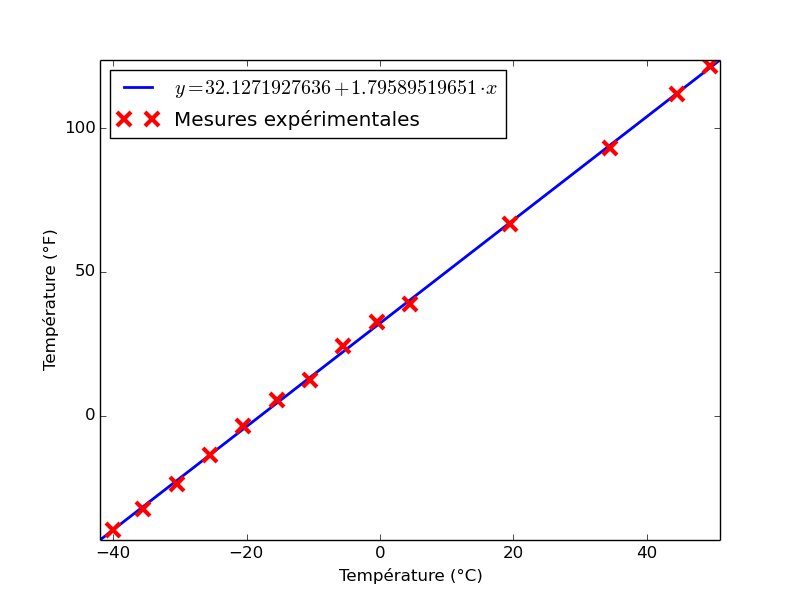
\includegraphics[width=\textwidth]{regression_temperature.png}
  \caption{Régression linéaire par moindres carrés entre les degrés Celsius et Farenheit.}
  \label{13systeme:fig:regression_temperature}
\end{center}
\end{figure}
%\clearslide{}
\subsection{Inconvénient}

La résolution par transposition amplifie les erreurs : $(A+\delta A)^T(A+\delta A)=A^TA+\delta 
A^TA+A^T\delta A+\delta A^T\delta A \cdots$.

Il existe des méthodes plus stables : utilisation de matrices orthogonales, de pseudo-inverses, 
décomposition QR ...

% \subsection{Matrices orthogonales}
% 
% On dira qu'une matrice $M\in \cM_{nm}(\R)$ est \emph{orthogonale} si
% l'application
% \begin{equation*}
%   \fct{\R^{m}}{\R^{n}}{x}{Mx}
% \end{equation*}
% préserve la norme $2$, i.e. $\forall x \in R^{n} \quad \norm{Mx}=
% \norm{M}$
% 
% %\clearslide{}
% Toute matrice orthogonale:
% \begin{enumerate}
% \item préserve les produits scalaires car $M(\vec{u}+\vec{v}) =
%   M\vec{u}+M\vec{v}$ et
%   \begin{equation*}
%     \vec{u}\cdot\vec{v} = \frac{1}{2}\p{\norm{\vec{u}+\vec{v}}^{2} - \norm{\vec{u}} - 
% \norm{\vec{v}}}
%   \end{equation*}
% \item préserve les angles car
%   \begin{equation*}
%     \cos (\vec{u},\vec{v}) = \frac{\vec{u}\cdot\vec{v}}{\norm{\vec{u}}\times\norm{\vec{v}}}
%   \end{equation*}
% \end{enumerate}
% 
% %\clearslide{}
% \subsection{Pseudo-inverse}
% 
% Étant donné une matrice $A\in \cM_{pq}(\R)$, on peut définir son
% \emph{pseudo-inverse de Moore-Penrose} $A^{+}$ (même si $A$ non
% inversible et même si $A$ non carrée).
% 
% C'est l'unique matrice vérifiant:
% \begin{enumerate}
% \item $A^{+} \in \cM_{pq}(\R)$
% \item $A A^{+} A = A$
% \item $A^{+} A A^{+} = A^{+}$
% \item $A A^{+}$ est une matrice orthogonale
% \item $A^{+} A$ est une matrice orthogonale
% \end{enumerate}
% 
% %\clearslide{}
% \subsection{Moindres carrés}
% 
% L'ensemble des vecteurs $x$ minimisant  $\norm{Ax-b}$ est le
% sous-espace affine $A^{+}b + \Ker A$.
% 
% Et parmi eux, $A^{+}b$ est le vecteur de norme minimale.
% 
% \subsection{Calcul du pseudo-inverse}
% 
% Il existe plusieurs méthodes de calculs. Les plus utilisées passent
% par une décomposition implicite ou explicite de la matrice $A$:
% \begin{description}
% \item[Décomposition $QR$] $A$ est mis sous la forme $QR$ où $R$ triangulaire supérieure et $Q$  
% orthogonale.
% \item[Décomposition en valeurs singulières]\footnote{En anglais,
%     Singular Value Decomposition, en abrégé SVD.}  $A$ est mis sous
%   la forme $U\Sigma V$ où $U$ et $V$ orthogonales et $\Sigma$ diagonale à
%   coefficients positifs ou nuls.
% \end{description}

%\clearslide{}
\section{Regard critique}
\subsection{Résumons}

On travaille sur une matrice carrée $A$ de taille $n$.

\begin{enumerate}
\item On veut parfois des valeurs de $n$ élevées: plusieurs milliers.
\item La complexité de ces méthodes est en général de l'ordre de la
  méthode du pivot: $\Theta(n^{3})$.
\item C'est l'ordre de grandeur du coût de la multiplication naïve.
\end{enumerate}

%\clearslide{}
Peut-on faire mieux?
\begin{itemize}
\item oui, il y a des algorithmes un peu plus
efficaces pour obtenir les mêmes décompositions (mais c'est délicat).
\item mais bien souvent en informatique, il vaut mieux se poser la
  question de la pertinence de ce qu'on fait.
\end{itemize}

%\clearslide{}
\subsection{Cadre physique}

\begin{enumerate}
\item interactions seulement entre des points proches
\item donc la matrice $A$ est creuse (une majorité de zéros).
\end{enumerate}

On peut améliorer la représentation des matrices et les algorithmes
d'addition et de multiplication pour en tirer parti.

Problème: le pivot de Gauss, aussi bien que les méthodes
\og{}efficaces\fg{} sur des matrices quelconques, basées sur des
décompositions des matrices  (LU, PLU, QR, \ldots{}), ont tendance à
remplir les matrices.

%\clearslide{}
\subsection{Méthodes plus adaptées aux matrices creuses}

Pour résoudre $Ax=b$ pour une matrice creuse,

Utilisation de méthodes itératives pour les matrices creuses:
\begin{enumerate}
\item on part d'une solution approchée;
\item on l'améliore;
\item revenir au point précédent tant que nécessaire.
\end{enumerate}
 
Intérêt de ces méthodes:
\begin{enumerate}
\item Pas besoin de calculer de nouvelles matrices (on reste sur des
  matrices creuses);
\item On améliore peu à peu une solution: impact des erreurs de calcul
  a priori plus faible.
\end{enumerate}

\section{Exercices}

Dans chaque exercice, on demande une valeur approchée du résultat. 

%\begin{exo}
  Résoudre le système 
  \begin{equation*}
    \bpm 5 & 8 & -2 \\ 3 & 1 & 5 \\ 0 & -2 & 6 \epm \times X = \bpm 21 \\ 16 \\ 10 \epm.
  \end{equation*}
%\end{exo}

%\begin{exo}
  On pose
  \begin{equation*}
    A = \bpm 3 & -2 & 5 \\ -4 & 1 & 1 \\ 2 & 3 & -2 \epm. 
  \end{equation*}
  En effectuant un seul calcul, résoudre simultanément les systèmes : 
  \begin{equation*}
    AX = \bpm 20 \\ -2 \\ -7 \epm,\quad AX = \bpm -21 \\ 23 \\ -1 \epm,\quad AX = \bpm -12 \\ 17 \\ 4 \epm,\quad AX = \bpm 6\\-2\\3\epm.
  \end{equation*}
%\end{exo}

%\begin{exo}
  Inverser la matrice 
  \begin{equation*}
    A = \bpm 5&-3&2&1&-1 \\3&6&8&1&-3 \\ 5&6&3&0&2 \\ 4&6&2&8&3 \\ -6&3&5&-1&-2 \epm.
  \end{equation*}
%\end{exo}

%\begin{exo}
  On considère les points de coordonnées 
  \begin{equation*}
    M_1 \bpm -5 \\ 11,67 \epm,\quad M_2 \bpm -2 \\ 4,52 \epm,\quad M_3 \bpm 1\\-0,15 \epm,\quad M_4\bpm 2 \\ -3,31 \epm.
  \end{equation*}
  On cherche à ajuster une droite affine sur le nuage de points $(M_1,M_2,M_3,M_4)$ par le critère des moindres carrés. Avec 
  \begin{equation*}
    A = \bpm 1 & -5 \\ 1 & -2 \\ 1 & 1 \\ 1 & 2 \epm, \quad X = \bpm \alpha \\ \beta \epm \quad\textrm{et} \quad B = \bpm 11,67 \\ 4,52 \\ -0,15 \\ -3,31 \epm,
  \end{equation*}
  déterminer $X$ minimisant la quantité 
  \begin{equation*}
    \norm{AX-B}. 
  \end{equation*}
  Produire une figure superposant les points $(M_1,M_2,M_3,M_4)$ et la droite d'équation $y = \alpha + \beta x $. 
%\end{exo}

%\begin{exo}
  On considère les points de coordonnées 
  \begin{equation*}
    M_1 \bpm -2 \\ 7,62 \epm,\quad M_2 \bpm -1 \\ 3,87 \epm,\quad M_3 \bpm 0 \\ 0,94 \epm,\quad M_4 \bpm 1\\1,56 \epm,\quad M_5\bpm 2 \\ 2,66 \epm.
  \end{equation*}
  On cherche à ajuster une courbe polynomiale de degré $2$ sur le nuage de points $(M_1,M_2,M_3,M_4,M_5)$ par le critère des moindres carrés. Avec 
  \begin{equation*}
    A = \bpm 1 & -2 & 4 \\ 1 & -1 & 1 \\ 1 & 0 & 0 \\ 1 & 1 & 1\\ 1 & 2 & 4\epm, \quad X = \bpm \alpha \\ \beta \\ \gamma \epm \quad\textrm{et} \quad B = \bpm 7,62 \\ 3,87 \\ 0.94 \\ 1,56 \\ 2,66 \epm,
  \end{equation*}
  déterminer $X$ minimisant la quantité 
  \begin{equation*}
    \norm{AX-B}. 
  \end{equation*}
  Produire une figure superposant les points $(M_1,M_2,M_3,M_4,M_5)$ et la courbe d'équation $y = \alpha + \beta x + \gamma x^2$. 
%\end{exo}

